\documentclass[a4paper]{report}
    
    \usepackage[english]{babel}
    \usepackage[utf8]{inputenc}
    \usepackage{amsmath}
    \usepackage{graphicx}
    \usepackage[colorinlistoftodos]{todonotes}



    % CUSTOM MARGIN AND PARAMETER
    \usepackage[a4paper, portrait, left=1.2in,right=1in,bottom=1in,top=1in]{geometry}

    \usepackage{sectsty}
    
    \sectionfont{\fontsize{12pt}{0}\selectfont}
    \subsectionfont{\normalfont \itshape \fontsize{12pt}{0}\selectfont}
    \subsubsectionfont{\normalfont \itshape \fontsize{12pt}{0}\selectfont}
    \paragraphfont{\fontsize{12pt}{0}\selectfont}
    \chapterfont{\fontsize{14pt}{0}\selectfont}

		

    \title{Quantum Hall effect report template}   

    \title{Backend and Analytics as a service}
    
    \author{Aditya and Shubham}
    
    \date{\today}
    
    \begin{document}
    
    \begin{titlepage}
      \maketitle 
    \end{titlepage}    
    
    \newpage
    \tableofcontents{}    

    \chapter {Introduction}
    
    \section{Preamble}
    \label{sec:introduction}    
    Technology driven solutions and analytics based decision making is the core of any business in the current scenario. Moreover, creation and integration of backend and frontend for a medium sized application requires 18 weeks of time comprising of 55 percent time in backend development and average cost ranging from \$8000 to \$50,000.  Moreover in today’s scenario, there is a business urge to include statistics and other analysis to make crucial profit decisions.Growth of Analytics just as a Service is expected to be  23.4 bn dollars by 2021, and that of Backend as a service will be 208.1 bn dollars. Thenceforth, there arises the need for providing the developers with an automated tool with integrated features of backend and analytics development which will ultimately act as a profit making job in terms of cost, time and other crucial factors.
    
    \section{Need of the project}
    \label{sec:theory}
    Developing the backend and analytics services at a single platform along with the minimization of the actual coding hours is the need of the hour; thereby increasing the throughput. At the same time, due to the digitization and the demand of analytics in business sector, there is a vast opportunity for the application developers to integrate analytics solution in their applications. 
    
    But for this, the developers have to perform tedious work which usually includes a lot of redundant and unproductive jobs (including the CRUD applications, etc.)  eventually increasing the development time and cutting down on various other important tasks like the front end development, rigorous testing, performing critical analysis, etc. 
    
    Using automated tools for performing and maintaining CRUD operations would ease the developer's task as it will reduce the latency caused by redundant or other housekeeping jobs like authentications/authorisation, third-party logins, etc.
    
    Also, considering the analytics, the developers have to spend a lot of time studying and working on the algorithms that seems to be feasible to the situation. This also reduces the scope of algorithm comparison for the feasibility and optimality as the developer has to spend a lot of time creating different algorithms and then performing analytics with their help; so usually they come up with a theoretically optimal algorithm than a practical and tested/compared optimal ones.
    \section{Problem Statement}
    Software solution providers face constant challenge to provide a cutting edge solution to their clients along with the minimization of cost and efforts. They tackle problems related to compatibility of various technologies and constant maintenance of the software. This has been done for a long time using conventional approach of complete software coding along with a dedicated maintenance cycle. The approach has been successful but their are a lot of redundant tasks which span across projects and the goal is to minimize these tasks which can be done with minimal or no coding.    
    \section{Objectives}
    The aim of the project is - \\
    \begin{itemize}
      \item {\textbf{Stops unnecessary stack development:} Instead of many developers being forced to recreate a stack for each mobile app they develop, a BAaS service can provide for much of their underlying processing needs. The main issue would then be connecting to an API; instead of spending hours developing customized stacks, that have to be re-created, changed, and reassembled to fit the needs of each of the different app platform. Developers can build just what they need on top of the existing structures, instead of starting from scratch each time.
      }}
      \item {\textbf{Allows for more accessibility: } If each app has the same underlying base, then BAaS has the potential to easily link apps across platforms. This has many benefits: from easier data sharing to better accessibility for cloud storage, a quicker spin-up time, and an overall better user experience.      
      }}
      \item {\textbf{Provides diverse outcomes from one model: } Think of BAaS like a "starter home." Each user starts off with the same basic elements and continues to add over those elements to create their own customized "home." However, the base elements of the house are all the same, other users have the potential to more easily understand and even interact with or fix the "house," creating a unified backend that has a better and stronger user base. Therefore, we are reducing the redundancy of writing the same code over applications.      
      }}
      \item {\textbf{Provide backend ready applications: } BAaS aims to provide the fastest way to build, deploy and manage a production application backend. To achieve this, BAaS provides a standardized architecture that  includes as much automation as possible.      
      }}
      \item {\textbf{Provide a one-stop platform for various analytics: } BAaS aims at providing a platform for directly implementing the various types of machine learning and data analytics algorithms and thus enables a comparative study of algorithms on same situation and so the user(developer) could eventually choosing the most optimal as per his considerations.      
      }}
    \end{itemize}


    \section{Solution Approach}
Various models are available for the development of a fully-fledged application as a developer. However taking the help of this project, the developer can have all the required functionalities and features as mentioned earlier.

As an approach to solving the problem, the developer will be provided with a software package which can be installed on the server. Various tools will be integrated and various APIs will be generated as the first step which will include the most necessary ones which are even crucial for a naive application like data APIs, auth APIs, logging and monitoring APIs and control APIs.
As a second step, various other APIs can be added by the developer which will facilitate in terms of providing fully functioning separate modules which can directly be used as end-points for their application.
The developer’s convenience to use these APIs will also be taken into consideration as in the form of providing simple and easy to use User Experience for the same.
As a parallel step, various analytical algorithms will also be developed to be provided to the developers as an on-the-go APIs/code. As a first step, we plan to integrate the most crucial 6-7 algorithms like of Classification, Clustering, Regression etc.
The user can can select from a number of algorithms available to make a fully functioning funnel whose entry point will have the live data stream and output being the final/live feed or report    
\section{Organisation of the Project Report}    
The report consists of a brief description of the problem as a whole and then a brief overview to the solution approach is provided. This is further elaborated by the use of the required lists of figures, tables, models, architecture and annexes which present the need, approach, enhancements in the pre-existing architecture and other detailed approach of the project. This is further followed by our methodology and approach used to implement the project.

Finally this is followed by a crisp summary of the project thereby proving its importance.

Chapter 1 provides introduction about the project, its need, problem statement, objectives and solution approach.
Chapter 2 is focused on the background of project which includes the area, available tools, hardware and software, the references used in the projects like the research papers and their limitations.
Chapter 3 includes detailed problem statement, requirement analysis, functional and nonfunctional requirements, feasibility study, and other required diagrams which better present the picture.
Chapter 4 includes the architectural diagrams, with the various design issues, architecture used, along with the insights of the various models, algorithms / approaches used.
Chapter 5 presents the conclusion of the report with specifying the various phase wise implementation of the project.

    
    
    \chapter {Background}
    Explain the experimental set-up here. Use a schematic picture (make it yourself in photoshop, paint, ...) to show how the components are connected. Briefly explain how a lock-in amplifier works.
    
    \section{Area,available tools and hardware and software}
    Show a graph of the longitudinal resistivity ($\rho_{xx}$) and Hall resistivity ($\rho_{xy}$) versus magnetic field, extracted from the raw data shown in figure \ref{fig:data}. You will have the link to the data in your absalon messages, if not e-mail Guen (guen@nbi.dk). Explain how you calculated these values, and refer to the theory.
    
    \begin{figure}
    \centering
    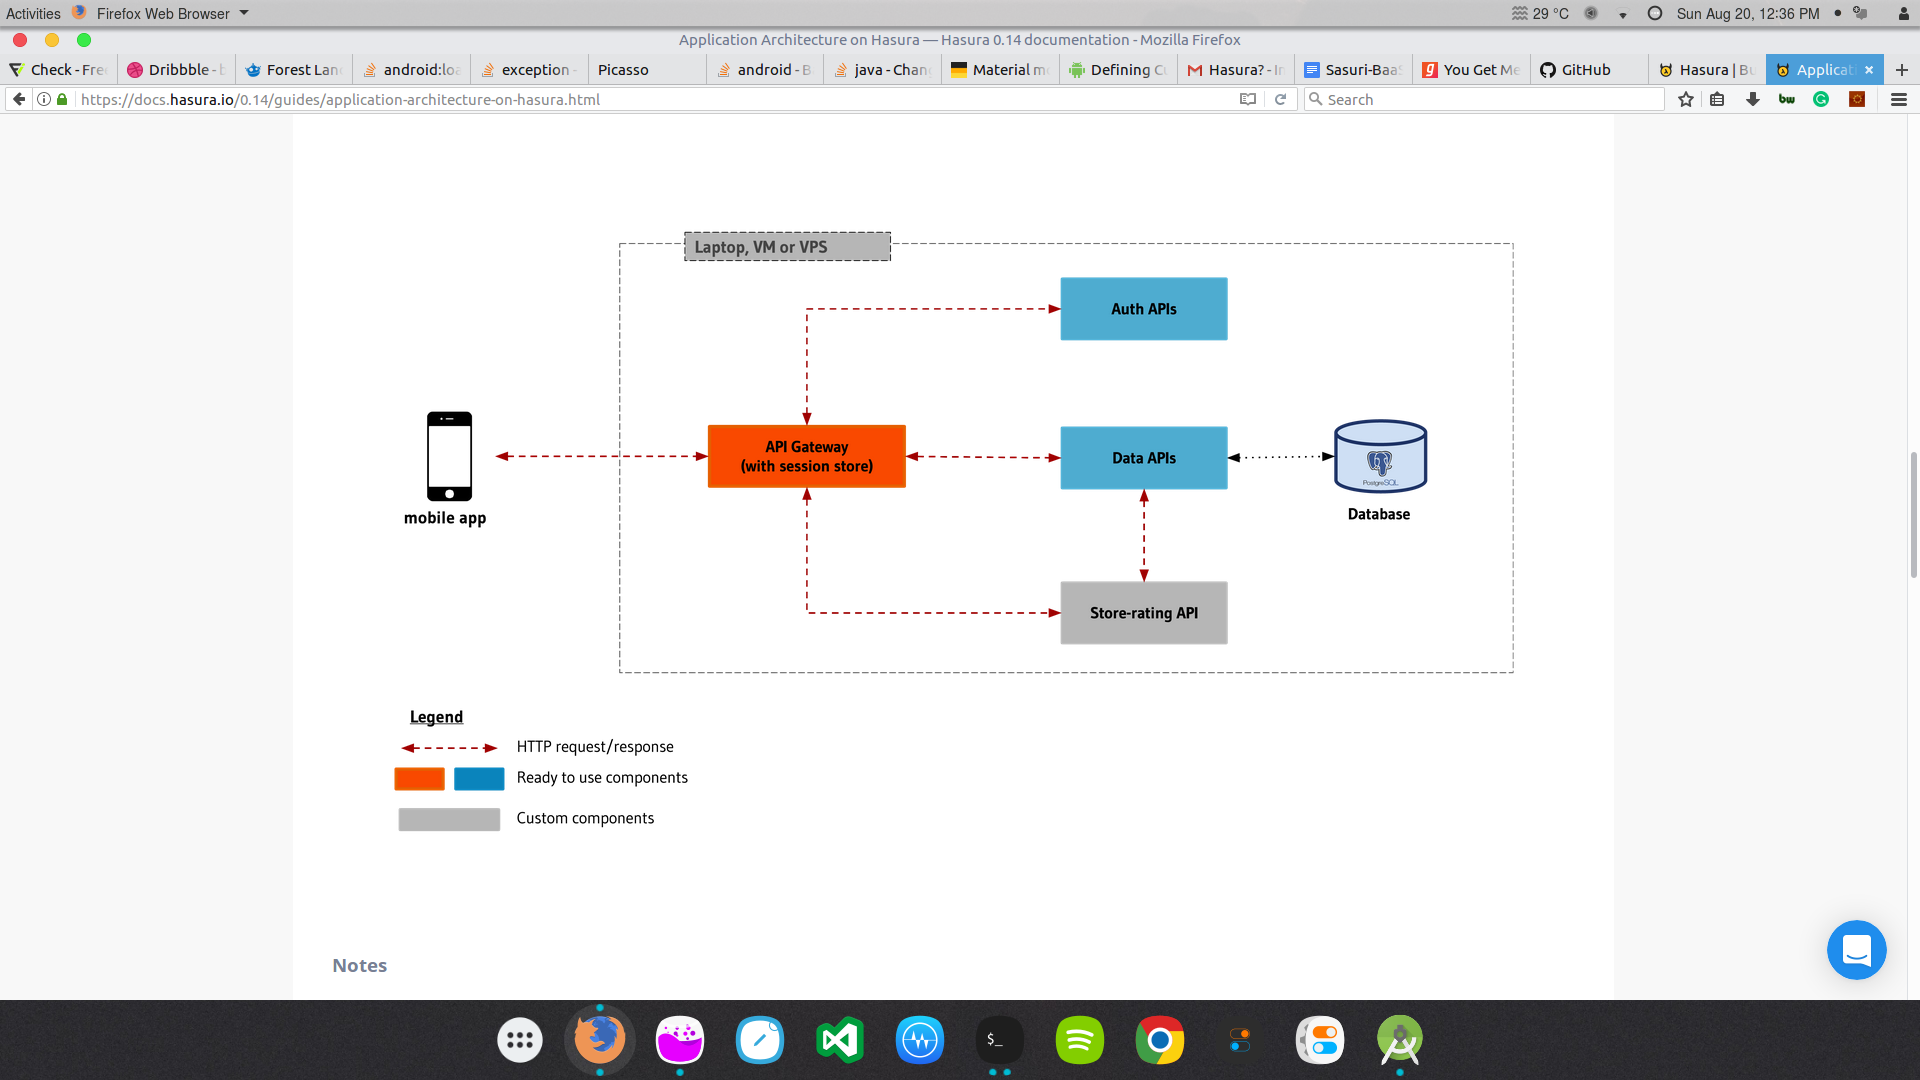
\includegraphics[width=1\textwidth]{test.png}
    \caption{\label{fig:data} Activity Diagram sample}
    \end{figure}
    
    \section{Literature review}
    Calculate the sheet electron density $n_{s}$ and electron mobility $\mu$ from the data in the low-field regime, and refer to the theory in section \ref{sec:theory}. Explain how you retrieved the values from the data (did you use a linear fit?).
    Round values off to 1 or 2 significant digits: 8.1643 ~= 8.2. Also, 5e-6 is easier to read than 0.000005.
    
    !OBS: This part is optional (only if you have time left).
    Calculate the uncertainty as follows: \newline $u(f(x, y, z)) = \sqrt{(\frac{\delta f}{\delta{x}} u(x))^{2} + (\frac{\delta f}{\delta{y}} u(y))^{2} + (\frac{\delta f}{\delta{z}} u(z))^{2}}$, where $f$ is the calculated value ($n_{s}$ or $\mu$), $x, y, z$ are the variables taken from the measurement and $u(x)$ is the uncertainty in x (and so on).
    
    \subsection{Area,available tools and hardware and software}
    Calculate $n_{s}$ for the high-field regime.
    Show a graph of the longitudinal conductivity ($\rho_{xx}$) and Hall conductivity($\rho_{xy}$) \textbf{in units of the resistance quantum} ($\frac{h}{e^{2}}$), depicting the integer filling factors for each plateau.
    Show a graph of the plateau number versus its corresponding value of $1/B$. From this you can determine the slope, which you use to calculate the electron density.
    Again, calculate the uncertainty for your obtained values.
    
    \subsection{Literature review}
    Discuss your results. Compare the two values of $n_{s}$ that you've found in the previous section. Compare your results with literature and comment on the difference. If you didn't know the value of the resistance quantum, would you be able to deduce it from your measurements? If yes/no, why?
    
    \chapter {Analysis}
    \section{Detailed Problem statement}
    \label{sec:theory}
    Here, explain the concept of a 2-DEG in GaAs/AlGaAs. What is a 2-DEG and why does it arise?
    \section{Requirement Analysis}
    Here, explain the concept of a 2-DEG in GaAs/AlGaAs. What is a 2-DEG and why does it arise?
    \subsection{Functional Requirement}
    Explain the classical Hall effect in your own words. What do I measure at $B=0$? And what happens if $B>0$? Which effect gives rise to the voltage drop in the vertical direction?
    \subsection{Non-Functional Requirement}
    Explain the IQHE in your own words. What does the density of states look like in a 2-DEG when $B=0$? What are Landau levels and how do they arise? What are edge states? What does the electron transport look like when you change the magnetic field? What do you expect to measure?    
    \section{Feasibility Study}    
    Explain a step-by-step recipe for fabrication here. How long did you etch and why? What is an Ohmic contact?
    \section{Diagram (as per our project problem)}
    a
    \begin{figure}
    \centering
    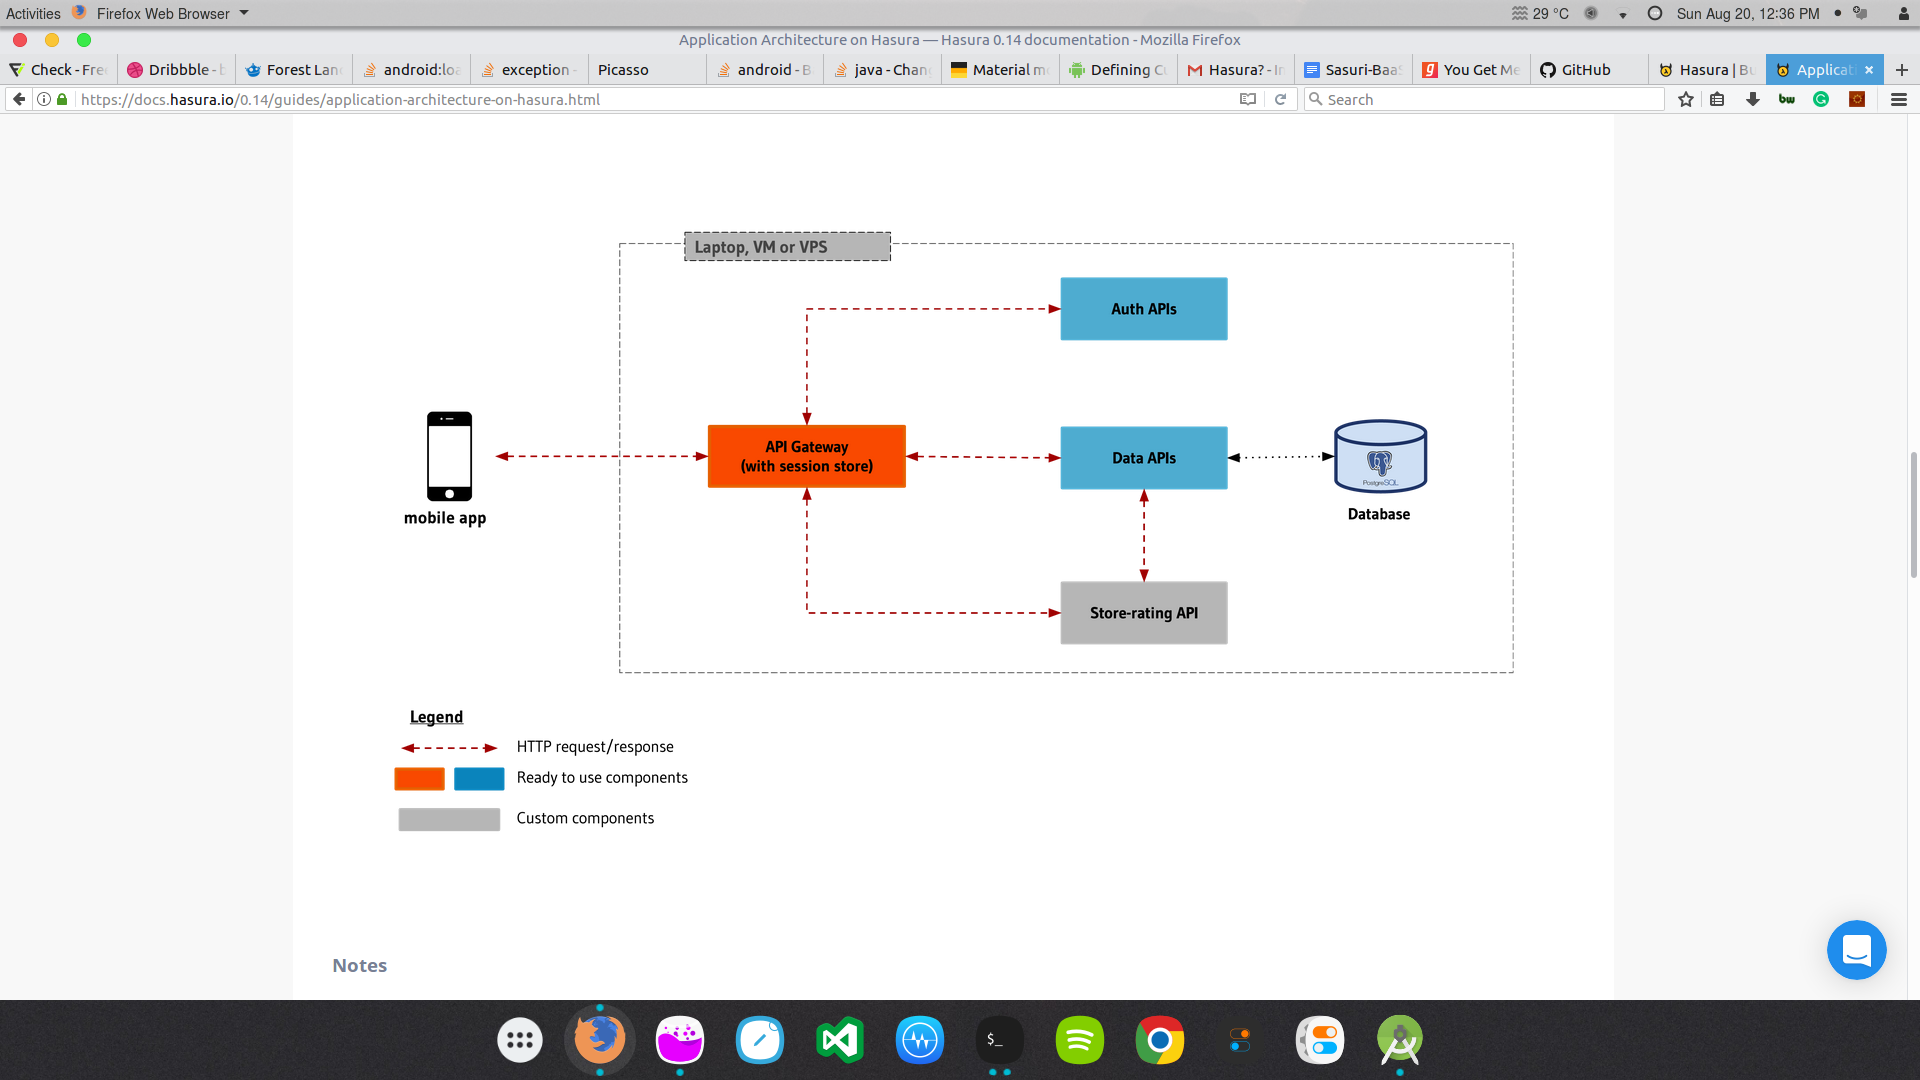
\includegraphics[width=1\textwidth]{test.png}
    \caption{\label{fig:data}Raw (unprocessed) data. Replace this figure with the one you've made, that shows the resistivity.}
    \end{figure}    
    
    \chapter {Architectural Diagrams}
    \section{Architectural Diagram. Discussion of moules}
    Architectural Designs
    \section{Algorithm Designed}
    Algorithm 
    \section{Diagrams}
    Diagrams

    \chapter {Conclusion}
    \section{Work carried out in phase 1}
    \begin{itemize}
      \item  Detailed study of Existing Systems
      \item  SRS(Software Requirement Specification)
      \item  Project Report and documentation
      \item  Finalised functional and nonfunctional requirements and features
      \item  Finalised our technology stack
    \end{itemize}
    \section{Work to be carried out in phase 2}
    \begin{itemize}
      \item  Creating User Interface and Configuring server
      \item  Implementation of the software package
      \item  Creating Endpoints for the algorithms
      \item  Implementation of analytical tools 
    \end{itemize}    


    \chapter{Sample items}
    \section{Some LaTeX tips}
    \label{sec:latex}
    \subsection{How to Include Figures}    
    First you have to upload the image file (JPEG, PNG or PDF) from your computer to writeLaTeX using the upload link the project menu. Then use the includegraphics command to include it in your document. Use the figure environment and the caption command to add a number and a caption to your figure. See the code for Figure \ref{fig:frog} in this section for an example.            
    \subsection{How to Make Tables}    
    Use the table and tabular commands for basic tables --- see Table~\ref{tab:widgets}, for example.    
    \begin{table}
    \centering
    \begin{tabular}{l|r}
    Item & Quantity \\\hline
    Widgets & 42 \\
    Gadgets & 13
    \end{tabular}
    \caption{\label{tab:widgets}An example table.}
    \end{table}    
    \subsection{How to Make Sections and Subsections}
    
    Use section and subsection commands to organize your document. \LaTeX{} handles all the formatting and numbering automatically. Use ref and label commands for cross-references.
    
    \subsection{How to Make Lists}
    
    You can make lists with automatic numbering \dots
    
    \begin{enumerate}
    \item Like this,
    \item and like this.
    \end{enumerate}
    \dots or bullet points \dots
    \begin{itemize}
    \item Like this,
    \item and like this.
    \end{itemize}
    \dots or with words and descriptions \dots
    \begin{description}
    \item[Word] Definition
    \item[Concept] Explanation
    \item[Idea] Text
    \end{description}
    
    We hope you find write\LaTeX\ useful, and please let us know if you have any feedback using the help menu above.

    

    \begin{thebibliography}{9}
    \bibitem{nano3}
    	Francis Gropengießer and Kai-Uwe Sattler,
      \emph{Database Backend as a Service: Automatic Generation, Deployment, and Management of Database Backends for Mobile Applications}.
			Available at https://link.springer.com/article/10.1007/s13222-014-0157-y
			
		\bibitem{nano3}
    	Francis Gropengießer and Kai-Uwe Sattler,
      \emph{Overview Of Backend as a Service (BaaS) White Paper}.
			Available at http://baas.apievangelist.com/2013/05/08/overview-of-backend-as-a-service-baas-white-paper/
			
								
		\bibitem{nano3}
			Balkan, A. 2012,
      \emph{What are the pros and cons of using a backend as a service?}.
			Available at https://www.quora.com/What-are-the-pros-and-cons-of-using-a-backend-as-a-service
		
		\bibitem{nano3}
			Backend as a Service (BaaS) Market Global forecast for 2020,
			Available at http://www.marketsandmarkets.com/PressReleases/baas.asp		
		
		\bibitem{nano3}
			Backendless website 2016,
      \emph{Database Backend as a Service: Automatic Generation, Deployment, and Management of Database Backends for Mobile Applications}.
			Available at https://backendless.com/what-is-backend-as-a-service/
	

		\bibitem{nano3}
			Ryan Goodrich,
      \emph{What is BaaS (Backend as a Service)}.
			Available at http://www.businessnewsdaily.com/4992-what-is-baas.html	
			
		\bibitem{nano3}
			Nguyen, T, 2016,
      \emph{Mobile Backend as a Service: The Pros and Cons of Parse
			Case company: SuperApp Oy}.
			Available at http://theseus.fi/bitstream/handle/10024/117483/Nguyen{\_}Phu.pdf?sequence=2
		
		\end{thebibliography}	
    \end{document}